% -*- TeX:UK -*-
\documentclass[10pt]{beamer}
\usetheme{metropolis}
%\useinnertheme{rectangles}
\setbeamercovered{%
still covered={\opaqueness<1->{15}},
again covered={\opaqueness<1->{40}}}

\hypersetup{colorlinks,linkcolor=black,urlcolor=brown,citecolor=brown}

\include{shared-tex/set-up-fonts-and-icons}

\usepackage{tikz}
\usetikzlibrary{positioning,fit,arrows}

\tikzset{
 big dot/.style
  = {circle, draw, inner sep=0pt, minimum size=3mm, fill=teal!50},
 a/.style
  = {node distance=4em, text width=0.1em, minimum height=4em},
 b/.style
  = {rectangle, draw, fill=gray!10, node distance=4em, text width=6em,
     text centered, rounded corners, minimum height=4em, thick},
 c/.style
  = {circle, draw, dashed, fill=orange!10, inner sep = 0pt, node distance=5em, text width=6em,
     text centered, thick},
 d/.style
  = {rectangle, draw, dashed, fill=red!10, node distance=4em, text width=6em,
     text centered, rounded corners, minimum height=4em, thick},
 l/.style
  = {draw, -latex, ultra thick},
 lr/.style
  = {draw, latex-latex, ultra thick, red},
 lb/.style
  = {draw, -latex, ultra thick, blue},
  lo/.style
  = {draw, -latex, ultra thick, orange},
  lg/.style
  = {draw, -latex, ultra thick, teal},
  mylabel/.style
  ={text width=6.5em, text centered},
 aa/.style
  = {node distance=4em, text width=0em, minimum height=0.5ex},
 ll/.style
  = {draw, {open triangle 45} -, thick},
 llb/.style
  = {draw, - triangle 45, thick, blue},
 llg/.style
  = {draw, - open triangle 45, thick, green},
  llt/.style
  = {draw, - open triangle 45, thick, teal},
 llr/.style
  = {draw, - triangle 45, thick, purple},
 llo/.style
  = {draw, - triangle 45, thick, orange}
}

\begin{document}

\title{PBIO-141\\Sensory and Physiological Ecology\\ of  Plants}
\subtitle{6: Responses to shading}
\author{Pedro J. Aphalo}
\date{January--February 2022}
\institute[Univ.\ of Helsinki]{M.Sc.\ in Plant Biology, University of Helsinki\\[2ex] \url{http://blogs.helsinki.fi/aphalo/}}


  \begin{frame}
    \maketitle
  \end{frame}

  \begin{frame}[c]
    \begin{center}
      \begin{small}
        \copyright 2006--2022 by Pedro J. Aphalo\\
        University of Helsinki, Finland.\\
        \textcolor{blue}{\url{http://blogs.helsinki.fi/senpep-blog/}}\\[2ex]
      \end{small}

      \begin{footnotesize}
        Sensory and Physiological Ecology of Plants slides by Pedro J. Aphalo are licensed under a Creative Commons Attribution-ShareAlike 4.0 International License.

      
\includegraphics[width=6em]{../figures/copyright/by-sa}\\[2ex]
      \end{footnotesize}
        
        \begin{scriptsize}
        Typeset in Lucida Sans, \textrm{Luicda Bright}, \texttt{Lucida Console} and Lucida Math. Icons from fonts ``WebHostingHub Glyphs'' (under SIL-Open Font License) from \url{https://www.webhostinghub.com/}; ``insect icons'' (free from \url{http://www.woodcutter.es/}); ``linea-basic-10'' and ``linea-weather-10'' (free from \url{https://github.com/linea-io}), ``Mini Pics Uprooted Twig'' and ``Mini Pics Uprooted Twig'' (commercial, from Image Club Graphics, Inc.). Plant icon as .svg by Abdul Wahhab (free from \url{NounProject.com}).

        Illustrations and text quoted from copyrighted sources is excluded from this license and their use should respect the original licenses.
        \end{scriptsize}
    \end{center}
  \end{frame}


  \begin{frame}
    \frametitle{Outline}
    \tableofcontents
  \end{frame}

\section{A new paradigm}

\begin{frame}
\frametitle{A new paradigm is emerging}
\textbf{An exciting time to study plants!!}
    \begin{itemize}
      \item Currently it is a very exciting time to study plants\ldots
      \item \ldots especially how their molecular biology, evolution and ecology are linked.
      \item We are in the middle of a paradigm shift\ldots
      \item \ldots for a long time we have disregarded/underestimated the central and complex role of plants' ``senses''.
      \item However, we should be open minded and use our imagination to understand plant life as it is\ldots
      \item \ldots rather than to project `human' features and qualities onto plants.
    \end{itemize}
\end{frame}

\section{Responses to (impending) shading}

\begin{frame}{Shade avoidance vs.\ tolerance strategies: $\neq$ ``goals''}
These are two extreme strategies with putative roles:
  \begin{itemize}
    \item Shade avoidance $\to$ compete for access to strong light
    \item Shade tolerance $\to$ efficiently use weak light
    \item Acclimated phenotypes are very different!
    \item Sources of information used in some combination are many:
    \item Cues: R:FR photon ratio, B:G photon ratio, blue light irradiance, UV irradiance, wind, touch, ethylene (signal?), including their temporal dynamics.
  \end{itemize}
\end{frame}

\begin{frame}{Shade avoidance vs.\ tolerance \Discussion 10 min}
  \begin{itemize}
  \item How do you expect avoidance and tolerance to work in practice?
  \item Can you think about clear-cut and less clear-cut cases?
  \item In which environments tolerance is likely to be better for fitness than shade avoidance?
  \end{itemize}
\end{frame}

\begin{frame}{Leaf size and angle, petiole length, chlorophyll}{}
    {\footnotesize End-of-day R or FR light (10 min/day),     \species{Petunia axillaris}, \autocite{Casal1987}\\}
    \includegraphics[angle=90,width=0.22\textwidth]{../photos/petunia_c}\hfil%
    \includegraphics[width=0.74\textwidth]{../figures/Petunia-Fig2}
\end{frame}

\begin{frame}{Stem elongation}
\footnotesize
    \begin{itemize}
        \item In sparse canopies `horizontal' light flux is important for anticipated sensing of neighbours.
        \item Growing internodes are a key site of perception.
    \end{itemize}

  \centering
  \includegraphics[width=0.8\linewidth]{photos/Pine-Nelder}\\
  \includegraphics[width=0.8\linewidth]{photos/Pine-Nelder-eos}

\end{frame}

\begin{frame}{Stem elongation}
\includegraphics[width=0.30\textwidth]{../photos/Birch-LEDs_photo}\hfil%
\includegraphics[width=0.65\textwidth]{../figures/Birch-LEDs_plot}\\
    {\small Irradiation with red or far-red light from LEDs at the growing internode (whole photoperiod),
    \species{Betula pendula}.}
    {\small \autocite[from][]{Aphalo2006}.}
\end{frame}

\begin{frame}{Leaf size, thickness and photosynthesis \Discussion}{}
    {\footnotesize High (HL) and low (LL) PAR, \species{Fuchsia magellanica} \autocite{AphaloEtAl1991}.\\}
    \includegraphics[width=0.34\textwidth]{../photos/fuchsia}%
    \includegraphics[width=0.65\textwidth]{../figures/Fuchsia-A-HL-LL}
\end{frame}

\begin{frame}{Stems position and length, apical dominance}{}
    {\footnotesize Sunlight, full and minus blue, \species{Medicago truncatula} Rai, Yan and Aphalo, unpublished.\\}
    \includegraphics[width=0.49\textwidth]{../photos/medic-full}\hfil%
    \includegraphics[width=0.49\textwidth]{../photos/medic-yellow}
\end{frame}

\nocite{Aphalo2021a}
  \begin{frame}[t,allowframebreaks]
    \frametitle{References}
    \printbibliography
  \end{frame}

%\begin{frame}{What is memory?}
%\begin{itemize}
%  \item Memory is storage of information in a way that can be recalled
%  \item Long-term `memory' in organisms is the genome
%  \item Medium-term `memory' is mostly in the epigenome
%  \item Shortest-term `memory' is in cell signalling and metabolic regulation
%  \item This is a useful oversimplification, so be careful!
%  \item The world cannot be described in three shades of grey...
%\end{itemize}
%\end{frame}
%
%\begin{frame}
%\frametitle{Plants store information}
%  \begin{itemize}
%    \item It has been shown that plants can `remember' past experiences.
%    \item For example the experience of cold is remembered (this is called vernalization).
%    \item There is also evidence that seeds of equal genotype, but that have formed under different environmental conditions, can produce plants with different phenology.
%    \item There is also some recent evidence of trans-generational memory, by which the environment under which parents have grown affects the behaviour of siblings.
%%    \item The capacity of plants to remember is dependent in many cases on epigenetic gene regulation, but other mechanisms like accumulation of metabolite precursors, or receptor proteins has also been suggested.
%  \end{itemize}
%\end{frame}
%
%\begin{frame}
%\frametitle{Communication within the plant}
%  \begin{itemize}
%    \item There is communication within plants.
%    \item The responses of different parts of an individual plant are coordinated.
%    \item This is not just a question of resource partition.
%    \item In plants there are hormones, small proteins, miRNAs, likely even electrical signals, moving from one place to another and transferring information.
%    \item For example a short time after irradiation of the shoot of a maize plant with ultraviolet radiation, gene expression changes both in the shoots and roots of the plant, and regulated genes are not all the same ones in both parts.
%    \item Soil drying is sensed by roots and plant hormones transfer this information to leaves (and leads to adjustment of stomatal opening).
%  \end{itemize}
%\end{frame}
%
%\begin{frame}
%\frametitle{Communication outwith the plant I}
%  \begin{itemize}
%    \item There is communication between plants.
%    \item The responses of different plants are to some extent coordinated.
%    \item This is not just a question of resource depletion.
%    \item Plants change the light environment (most likely a cue) allowing the detection of neighbours before competition for light starts.
%    \item Plants can recognize their own roots as different from those of neighbours and adjust growth based on this.
%  \end{itemize}
%\end{frame}
%
%\begin{frame}
%\frametitle{Communication outwith the plant II}
%  \begin{itemize}
%    \item Plants emit volatile metabolites that work as `alarm signals', informing other plants and other parts of the same plant, of for example impending attack by herbivore insects.
%    \item Plants emit volatile metabolites that work as `alarm signals', informing the predators of the herbivores that there are insects to be eaten.
%    \item It has been proposed, but not demonstrated, that plants when eaten by herbivore insects can produce UV-absorbing pigments that `tag' the attacked leaves making them easier for predator birds to find.
%  \end{itemize}
%\end{frame}
%
%\begin{frame}
%\frametitle{Communication outwith the plant III}
%  \begin{itemize}
%    \item There is current research on signaling between roots through the soil: for example closure of stomata in unstressed plants when they partially share the rooting space with salt stressed plants. The phenomenon has been demonstrated, but the mechanism is still under investigation, but release of the plant hormone ABA seems to be involved.
%    \item Research on the synchronization of other responses like flowering has shown that communication through roots is used by some species.
%    \item Fitness advantages of synchronization are in many cases obvious\ldots
%    \item \ldots and analyses explaining how altruism could have evolved exist, for example in birds and even in bacteria.
%\end{itemize}
%\end{frame}
%
%\begin{frame}
%  \frametitle{Self vs.\ alien recognition: What is the evidence?}
%  \begin{itemize}
%    \item Roots in the soil grow differently when near another root of the same plant than
%    when near roots of a different plant (even if the two plants have the same genotype).
%    \item There is keen recognition by shoots dependent on light perception (plants respond
%    differently depending on the species of the neighbours).
%  \end{itemize}
%\end{frame}
%


%\section{General discussion}

\begin{frame}
\frametitle{Environmental correlations and forecasting \Discussion}

\textbf{Can plants `predict' the arrival of the cold season?\\
 What sources of information do they use?}

    \centering
    \includegraphics[height=0.75\textheight]{../photos/winter}
\end{frame}

\begin{frame}
\frametitle{Environmental correlations and forecasting \Discussion}

\textbf{Can plants `predict' the arrival of the spring?\\
 What sources of information do they use?}

    \centering
    \includegraphics[height=0.75\textheight]{../photos/spring}
\end{frame}

\begin{frame}
\frametitle{Environmental correlations and forecasting \Discussion}

\textbf{Can plants emit `signals' for their benefit?\\
What are the signals used to attract pollinators?}

    \centering
    \includegraphics[height=0.75\textheight]{../photos/bumblebee}
\end{frame}

\begin{frame}
\frametitle{Environmental correlations and forecasting \Discussion}

\textbf{Can plants emit `signals' for their benefit?\\
What are the signals used to enlist ``helpers'' for seed dispersal?}

    \centering
    \includegraphics[height=0.75\textheight]{../photos/berry_eater}
\end{frame}

\begin{frame}
\frametitle{Environmental correlations and forecasting \Discussion}

\textbf{Can plants emit signals to deceive other organisms?\\
How does mimicry work?}

    \centering
    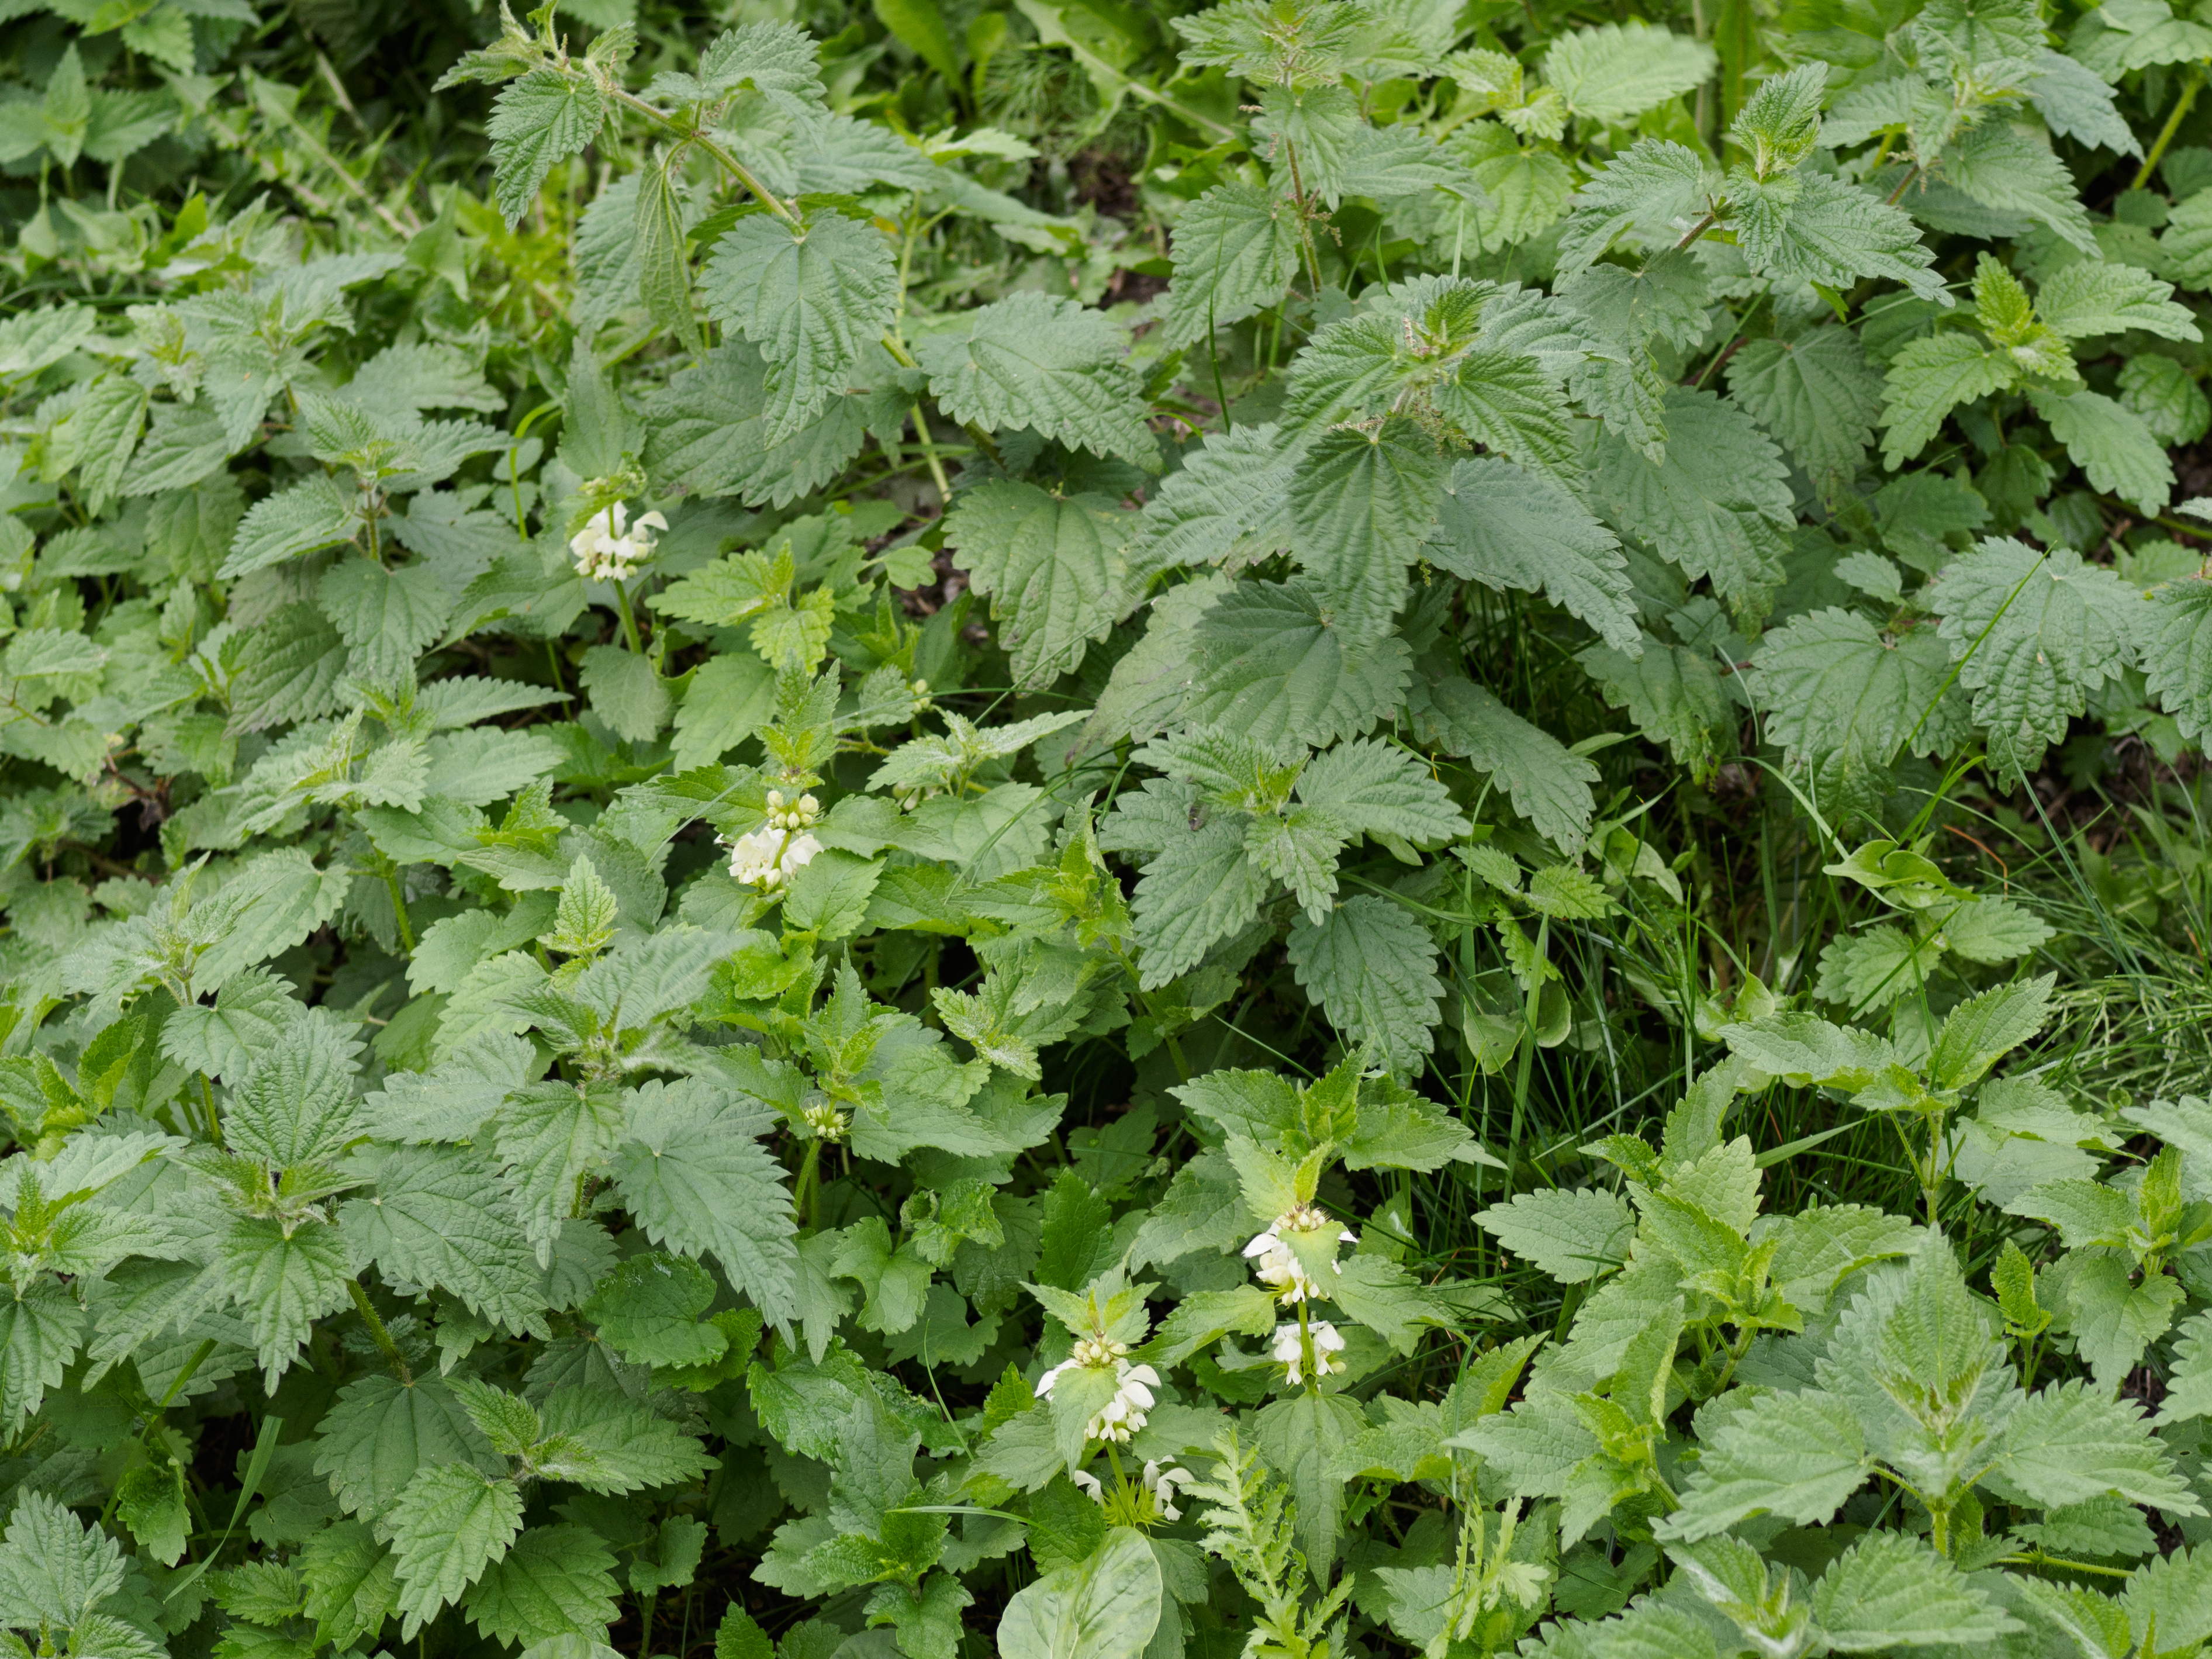
\includegraphics[height=0.75\textheight]{../photos/nettle}
\end{frame}

\begin{frame}
\frametitle{Environmental correlations and forecasting \Discussion}

\textbf{Can plants `generate' environmental correlations for their benefit?\\
How does release of organic volatile compounds create a correlation?}

    \centering
    \includegraphics[height=0.7\textheight]{../photos/aphids}
\end{frame}

\begin{frame}
\frametitle{Symbioses: ectomycorrhizas \Discussion}

\textbf{Do symbioses involve communication?}

    \centering
    \includegraphics[height=0.75\textheight]{../photos/dia3}
\end{frame}

\end{document}
